\documentclass[12pt, oneside]{article}
\usepackage{geometry}                		% See geometry.pdf to learn the layout options. There are lots.
\geometry{letterpaper} 
\usepackage{amsmath}
\usepackage{amsthm}
\usepackage{amssymb}
\usepackage{graphicx}
\usepackage{color}
\usepackage{float}
\usepackage{subfig}
\usepackage[flushleft]{threeparttable}
\usepackage{gensymb}
\usepackage{multirow}
\usepackage[dvipsnames]{xcolor}
\newcommand{\BibTeX}{\textsc{Bib}\TeX}
%opening
\title{spectcorr}
\author{}

\begin{document}

\section{Probibility Density Function}

The probibility density function can be used to evaluate the likeliness that a value will fall in a range, this is done by taking the 
intergral over a range of values. For example in figure 1 you would find that at any given point in time there is about a 33\% chance that the pressure would fall between
0 and 1.

\begin{figure}[H]
\centering
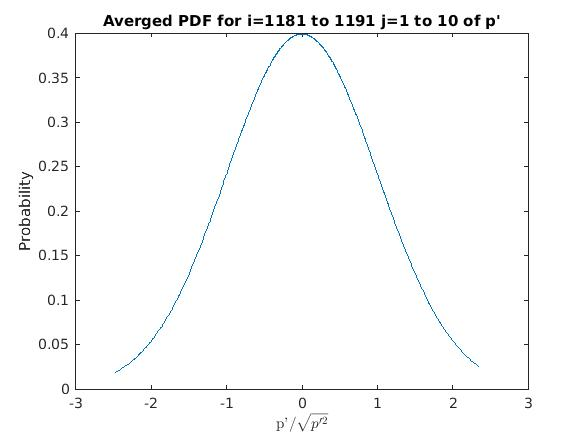
\includegraphics[width=0.5\textwidth]{FIGS/PDF_Plot.jpg}

\caption{{\footnotesize PDF Plot}}
\label{fig: } 
\end{figure}

The PDF functionality of spectcorr defines the fluctionations as the differnce from the mean value of a data set so that
\[x'(t)=x(t)-mean(dataset of x)\]

Before calculating the PDF the value is scaled with the datasets root mean squared,$\sqrt{\sum x'(t)^2}$ , and then plugged into the PDf in order to generate a plot.
For this code a Guassian distubution was used, so the function is \[f(x)= \dfrac{1}{(\sqrt{2\pi}\sigma)}exp[-\dfrac{(x-\mu)^2)}{2\sigma^2}]\]
Where \(\sigma\) is the standard deviation and \(\mu\) is the mean.

\section{Using the PDF function}


In order to use the code fill in the filepath so that the code has a path to your data and set icalPDF to 1.
Next define the index ranges you want to pull data from and the number of points in the time domain, ntpoint. 
Lastly fill the information about your DNS file.

Then run the code and 2 plots will be generated. The first will be a plot of each node locations PDF, while the second will be a plot of the PDF for all node points averaged together.
Additionally if raw data is desired, the averaged PDF outputs are stored in AvgPDF and the nodal PDF data is stored in PDFvalue.




\end{document}